\documentclass[12pt, reqno]{amsart}
\usepackage{geometry, setspace, amsmath}                % See geometry.pdf to learn the layout options. There are lots.
\geometry{a4paper}                   % ... or a4paper or a5paper or ... 
%\geometry{landscape}                % Activate for for rotated page geometry
%\usepackage[parfill]{parskip}    % Activate to begin paragraphs with an empty line rather than an indent
\usepackage{graphicx}
\usepackage{amssymb}
\usepackage{epstopdf}
\DeclareGraphicsRule{.tif}{png}{.png}{`convert #1 `dirname #1`/`basename #1 .tif`.png}



\begin{document}

\onehalfspacing

\section*{An Empirical Example: US Unemployment}

In this section, we revisit the empirical application in Hansen (1997), who used threshold autoregressive models for the US unemployment rate. 
Hansen (1997) measured unemployment among males age 20 and over and estimated his threshold model with the first-differenced series, say $\Delta y_t$, to avoid nonstationarity. The leg length in the autoregressive model was $p=12$ and his preferred threshold variable was 
$q_{t-1} = y_{t-1} - y_{t-12}$. In this section, we investigate the usefulness of a macro factor obtained form a large macro dataset.
In particular, we use the first factor, say $F_t$, of Ludvigson and Ng (2009) among eight common factors in their paper.
The first factor not only explains the largest fraction of the total variation in their panel data set but also loads heavily on employment, production, and so on. They call it a real factor and thus it is a great candidate for explaining the unemployment rate. 
We consider three different specifications for $f_t$: (1) $f_{1t} = (q_{t-1}, -1)$, (2) $f_{2t} = (F_{t-1}, -1)$, and (3) $f_{3t} = (q_{t-1}, F_{t-1}, -1)$.
That is, the first specification of $f_t$ corresponds to Hansen (1997), the second one  uses the first factor only, and the third case includes both. 
We combined the updated estimates of the first factor, which are available on Ludvigson's web page,
with Hansen's data, yielding a monthly sample from March 1960 to July 1996  for our estimation purpose. 

Table \ref{table-hansen97} reports the parameter estimates of regression coefficients and their  heteroskedasticity consistent standard errors for each of three specifications. It also shows the goodness of fit by reporting the average of squared residuals and the results of regime classification by showing the proportion between
the NBER recession indicators and regime indicators using three different specifications.   
Figure \ref{fig-hansen97} gives the graphical representation of regime classification. 

\begin{table}[htp]
\caption{Estimation Results}
\begin{center}
\begin{tabular}{lrrrrrr}
\hline\hline
Specification     & \multicolumn{2}{c}{(1)} & \multicolumn{2}{c}{(2)} & \multicolumn{2}{c}{(3)} \vspace*{1ex} \\ 
    & \multicolumn{2}{c}{$f_{1t} = (q_{t-1}, -1)$} & \multicolumn{2}{c}{$f_{2t} = (F_{t-1}, -1)$} & \multicolumn{2}{c}{$f_{3t} = (q_{t-1}, F_{t-1}, -1)$} \vspace*{1ex} \\ 
                  &   Estimate & Std. Err. &   Estimate & Std. Err.  &   Estimate & Std. Err. \\ 
\hline
\\
Regime 1          & \multicolumn{2}{c}{$q_{t-1} \leq 0.302$} & \multicolumn{2}{c}{$F_{t-1} \leq -0.28$} & \multicolumn{2}{c}{$q_{t-1} + 3.55 F_{t-1}$} \\
        &  & & & & \multicolumn{2}{c}{$\leq -1.60$} \vspace*{1ex} \\
Intercept         &  -0.0214   &  0.0126 & -0.0255  &  0.0101 &   -0.0294   &   0.0101   \\
$\Delta y_{t-1}$  &  -0.1696   &  0.0640 & -0.1182  &  0.0629 &   -0.1628   &   0.0601   \\
$\Delta y_{t-2}$  &   0.0382   &  0.0650 &  0.0774  &  0.0558 &    0.0264   &   0.0600   \\
$\Delta y_{t-3}$  &   0.1896   &  0.0587 &  0.2097  &  0.0645 &    0.1933   &   0.0520   \\
$\Delta y_{t-4}$  &   0.1399   &  0.0630 &  0.1039  &  0.0523 &    0.1445   &   0.0552   \\
$\Delta y_{t-5}$  &   0.0858   &  0.0749 &  0.0622  &  0.0600 &    0.0699   &   0.0656   \\
$\Delta y_{t-6}$  &   0.0214   &  0.0653 &  0.0193  &  0.0558 &    0.0177   &   0.0613   \\
$\Delta y_{t-7}$  &   0.0318   &  0.0678 & -0.0268  &  0.0596 &    0.0174   &   0.0613   \\
$\Delta y_{t-8}$  &   0.0402   &  0.0599 & -0.0006  &  0.0617 &    0.0103   &   0.0626   \\
$\Delta y_{t-9}$  &  -0.0667   &  0.0663 & -0.0766  &  0.0660 &   -0.0637   &   0.0656   \\
$\Delta y_{t-10}$ &  -0.0540   &  0.0640 & -0.0120  &  0.0559 &   -0.0467   &   0.0575   \\
$\Delta y_{t-11}$ &   0.0782   &  0.0568 &  0.0162  &  0.0529 &    0.0196   &   0.0528   \\
$\Delta y_{t-12}$ &  -0.0899   &  0.0641 & -0.1216  &  0.0576 &   -0.1224   &   0.0572   \\
\hline
\\
Regime 2          & \multicolumn{2}{c}{$q_{t-1} > 0.302$} & \multicolumn{2}{c}{$F_{t-1} > -0.28$} & \multicolumn{2}{c}{$q_{t-1} + 3.55 F_{t-1}$} \\
        &  & & & & \multicolumn{2}{c}{$> -1.60$} \vspace*{1ex} \\
%
%Regime 2          & \multicolumn{2}{c}{$q_{t-1} > 0.302$}  & \multicolumn{2}{c}{$F_{t-1} > -0.28$} & \multicolumn{2}{c}{$q_{t-1} + 3.55 F_{t-1} > -1.60$} \vspace*{1ex} \\
Intercept         &   0.0876   &  0.0375  &  0.0509  &  0.0560  &    0.1893   &    0.0576   \\
$\Delta y_{t-1}$  &   0.2406   &  0.1179  &  0.3671  &  0.2011  &    0.2937   &    0.1665   \\
$\Delta y_{t-2}$  &   0.2455   &  0.0932  &  0.2198  &  0.1634  &    0.1420   &    0.1279   \\
$\Delta y_{t-3}$  &   0.1283   &  0.1038  &  0.0936  &  0.1563  &    0.1042   &    0.1549   \\
$\Delta y_{t-4}$  &  -0.0222   &  0.1033  & -0.0053  &  0.1883  &   -0.1035   &    0.1690   \\
$\Delta y_{t-5}$  &  -0.0272   &  0.1104  & -0.1804  &  0.2188  &   -0.0723   &    0.1868   \\
$\Delta y_{t-6}$  &  -0.0851   &  0.1083  & -0.0500  &  0.2125  &   -0.0821   &    0.1400   \\
$\Delta y_{t-7}$  &  -0.1562   &  0.1057  & -0.0297  &  0.2027  &   -0.1853   &    0.1443   \\
$\Delta y_{t-8}$  &  -0.0372   &  0.1357  &  0.0021  &  0.2923  &   -0.1214   &    0.2038   \\
$\Delta y_{t-9}$  &   0.0991   &  0.1358  &  0.0754  &  0.1754  &   -0.0861   &    0.1475   \\
$\Delta y_{t-10}$ &   0.1149   &  0.1125  &  0.0445  &  0.1574  &    0.0392   &    0.1426   \\
$\Delta y_{t-11}$ &  -0.1012   &  0.1256  &  0.1872  &  0.1995  &   -0.0307   &    0.1840   \\
$\Delta y_{t-12}$ &  -0.4440   &  0.1144  & -0.2269  &  0.1668  &   -0.3807   &    0.1542   \\
\hline
\multicolumn{7}{l}{Avg. of squared residuals} \\
$(T^{-1} \sum_{i=1}^T \widehat{\varepsilon}_t^2)$          & \multicolumn{2}{c}{0.0264}  & \multicolumn{2}{c}{0.0272} & \multicolumn{2}{c}{0.0252} \vspace*{1ex} \\
\hline
\multicolumn{7}{l}{Proportion of matches between NBER recession dates and threshold estimates} \\
         & \multicolumn{2}{c}{0.807}  & \multicolumn{2}{c}{0.894} & \multicolumn{2}{c}{0.896} \vspace*{1ex} \\
\hline
\end{tabular}
\end{center}
\label{table-hansen97}
\end{table}




\begin{figure}[htbp]
	\caption{Regime Classification}
	\label{fig-hansen97}
	\begin{center}
		\graphicspath{ {plot/} }
		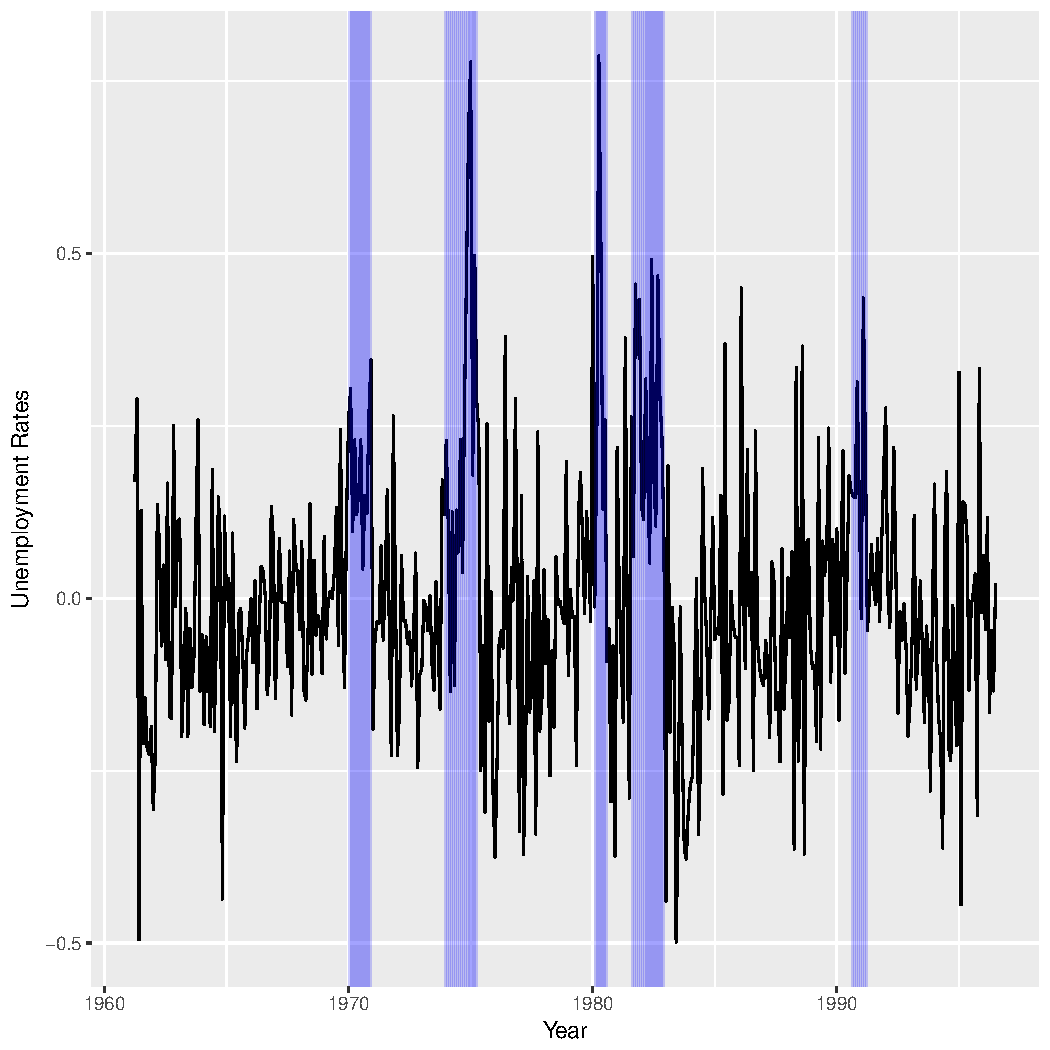
\includegraphics[scale=0.37]{UR_nber.pdf} 
		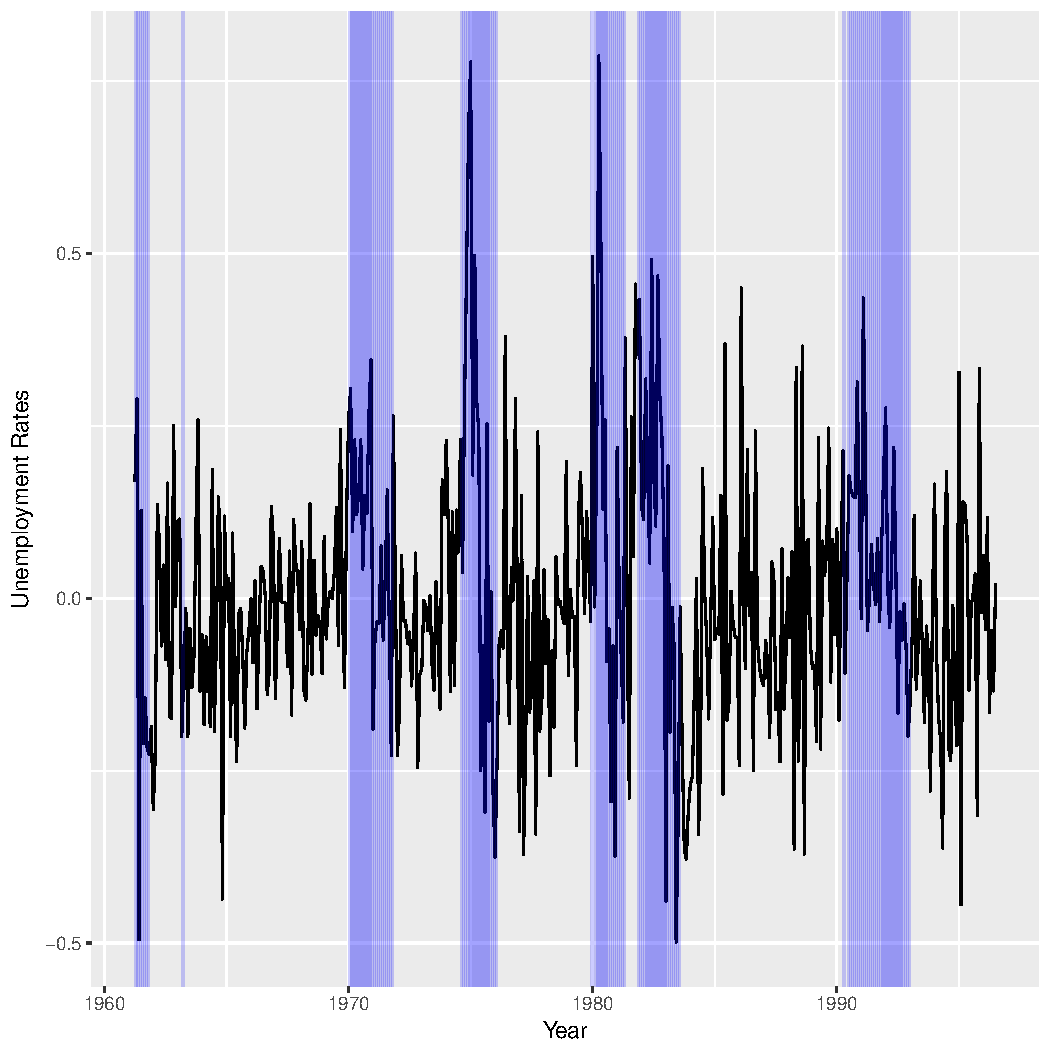
\includegraphics[scale=0.37]{UR_hansen.pdf}
		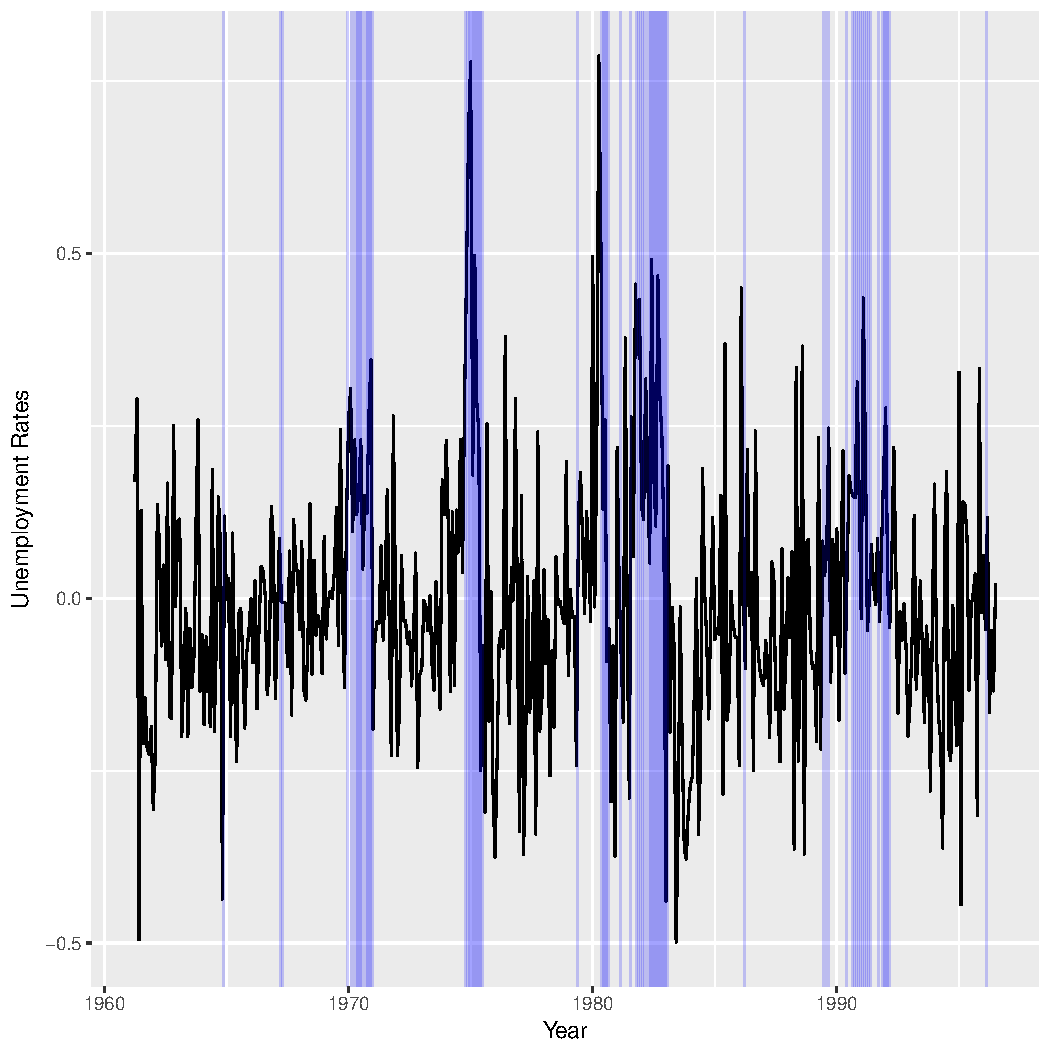
\includegraphics[scale=0.37]{UR_F1.pdf}
		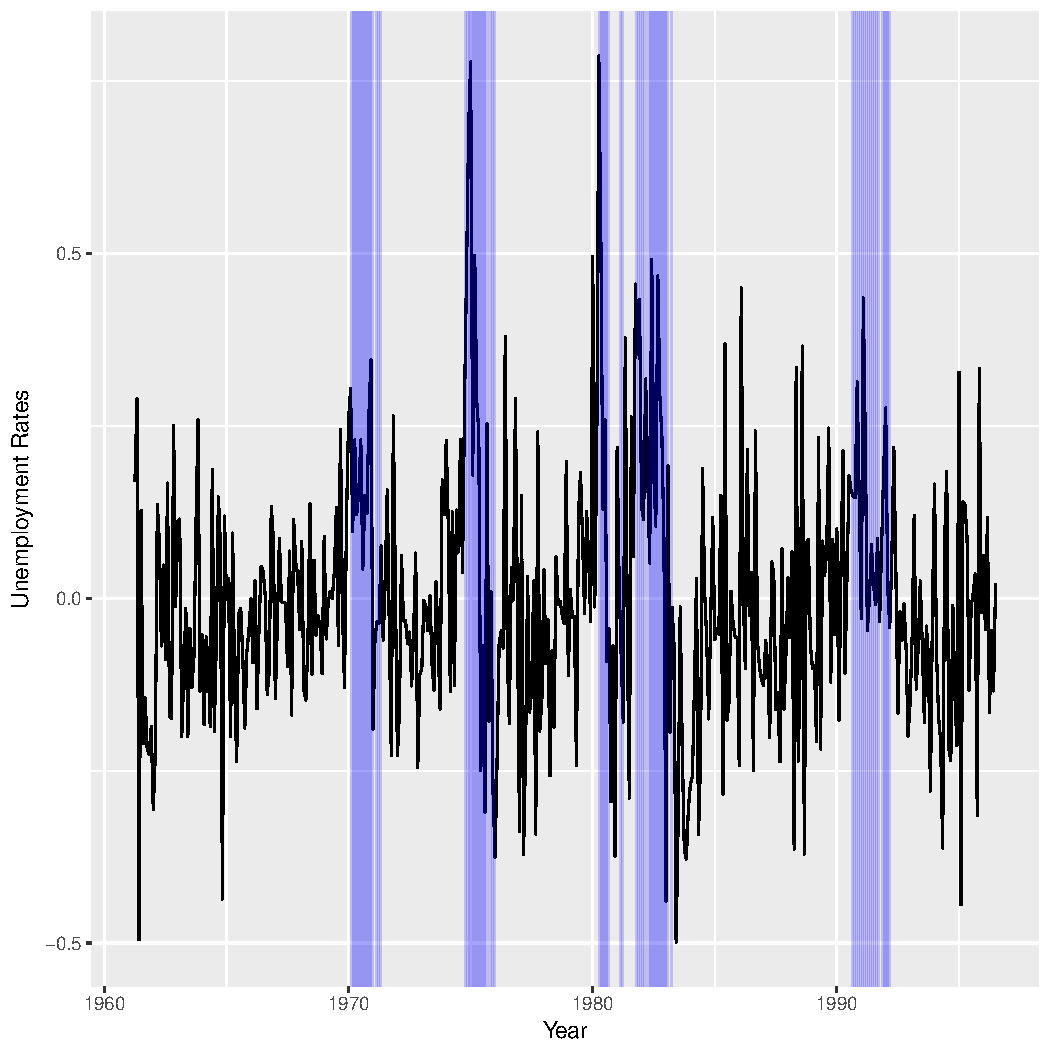
\includegraphics[scale=0.37]{UR_all.pdf}
	\end{center}

\parbox{6in}{Note. The top left panel shows NBER recession dates in the shaded area, 
the top right panel displays regime 1 with specification (1),
and
the bottom left and right panels show regime 1 with specifications (2) and (3), respectively.}
\end{figure}




\end{document}  


